\subsection{Embedded Software}
This section will cover how we plan to design the software running on our sensor node's microcontroller. Due to the need to run various different tasks in parallel, we will be utilizing FreeRTOS to aid in more effectively scheduling them. This design will require different tasks for handling the reading in of data from each sensor periodically, managing the battery and power subsystem, and sending any collected data to the internet over LoRaWAN.

\subsubsection{Managing Sensors}
Our software will require a task to control the different sensors and to manage the data received from them. To meet our goal of calculating the AQI, we will need to periodically take a measurement from each of the sensors. Some sensors will have a different measurement period than others. In addition, some sensors will take different amounts of time to warm-up and become ready to take measurement. This indicates that we will need to have a different FreeRTOS task dedicated to each sensor.

Each task will be independent, however, they will essentially all have the same flow. Each task will start in a sleep state and will remain there for a configurable amount of time. Then, the task will wake up the sensor to take a measurement. In addition, a timestamp will be appended to the data to document the measurement and assist with calculating the AQI. Finally, the task will request to be added to the so-called send queue. This send queue will be used to manage data and determine when to send it to the server over LoRaWAN. This task control flow can be seen in Figure \ref{fig:measurement-flow}. As shown, there are three tasks, one for each sensor in our design.

\begin{figure}[H]
    \centering
    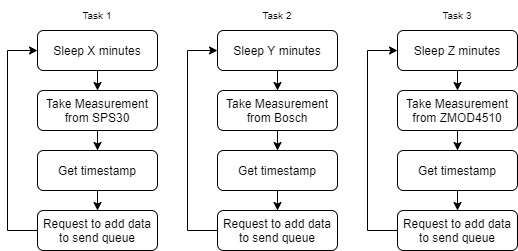
\includegraphics[width=6in]{figures/measurement-flow.png}
    \caption{A flowchart demonstrating how the software will create tasks for taking measurements from each sensor}
    \label{fig:measurement-flow} 
\end{figure}

\subsubsection{Sending Collected Data Over LoRaWAN}
Our software will require a task to manage how data collected from the sensors is sent to the server over LoRaWAN. One of the structures we decided to use to accomplish this is a queue. This queue will help optimize how and when data is sent from the sensor node. This will ensure that more data is sent together to optimize power consumption. In addition by adding this queue, it helps with the overall architecture of the design by further abstracting the sending of the data away from the collection of the data.

Our proposed queue will function by waiting for data to arrive from the sensors. Once one of the tasks controlling taking measurements from the sensors requests that data be added to the queue, the software will check if the queue is currently full. If the queue is full, all of the data currently in the queue will be sent and then the data being requested to be added to the queue will then be added. Otherwise, if the queue is empty, the data will be added immediately. In addition, we will have a timer running that will periodically empty the queue. This will ensure that the queue does not get stuck in a state where it never sends previously collected data because it is not receiving new data. A flowchart demonstrating how our proposed queue will function can be found in Figure \ref{fig:queue-diagram}.

\begin{figure}[H]
    \centering
    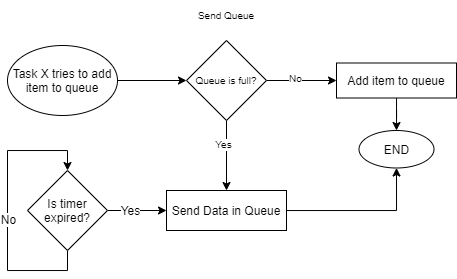
\includegraphics[width=6in]{figures/queue-diagram.png}
    \caption{A flowchart demonstrating how a queue will be used to manage sending data from the sensor node to the server over LoRaWAN}
    \label{fig:queue-diagram} 
\end{figure}

\subsubsection{Managing System Power}
Our software will require a task that manages how power is used in the system. This will alow the microcontroller to do things, such as dropping to different levels of low-power modes depending on how much power is available. To do this, the microcontroller will receive input from the charging controller IC that contains various information about the current state of the battery. Based on the charging controller we have selected, these states are low battery output/currently charging, fully charged, and power on.